\documentclass{emulateapj}
%\documentclass[12pt,preprint]{aastex}

\usepackage{graphicx}
\usepackage{float}
\usepackage{amsmath}
\usepackage{epsfig,floatflt}



\begin{document}

\title{Project 4}

\author{Christer Dreierstad}

\email{chrisdre@student.matnat.uio.no}

\altaffiltext{1}{Institute of Physics, University of
  Oslo, P.O.\ Box 1029 Blindern, N-0315 Oslo, Norway}


%\date{Received - / Accepted -}

\begin{abstract}

\end{abstract}
\keywords{computational science: Ising model  --- methods: Metropolis, Monte Carlo}

\section{Introduction}
\label{sec:introduction}
To study the phase transitions of a magnetic system we consider the Ising model for a two-dimensional system with a finite lattice size. The particles (spins) that make up the crystal (lattice) can take two values representing spin up or down. The energy of the lattice can then, by the Ising model, be found by
%
\begin{gather*}
    E = -J\sum_{< kl >}^N s_k s_l,
\end{gather*}
%
when there is no external magnetic field applied to the system. The coupling constant J will be set to 1, which means we are studying a ferromagnetic interaction between the spins that make up the lattice. Since the coupling constant is dependent upon the material we study, setting this to 1 allows for a general model. For studying the phase transition we consider the  Metropolis algorithm, a Markov chain Monte Carlo method (MCMC). 

\section{Method}
\label{sec:method}
h

The two-dimensional binary Ising model has analytical expectation values. 

\begin{deluxetable}{cccc}
\tablewidth{0pt}
\tablecaption{\label{tab:results}}
\tablecomments{....}
\tablecolumns{4}
\tablehead{Spins up  & Degeneracy & Energy & Magnetic moment}
\startdata
4 & 1 & -8J & 4 \\
3 & 4 & 0 & 2 \\
2 & 4 & 0 & 0 \\
2 & 2 & 8J & 0 \\
1 & 4 & 0 & -2 \\
0 & 1 & -8J & -4
\enddata
\end{deluxetable}


\section{Results}
\label{sec:results}

\begin{figure}[H]
{{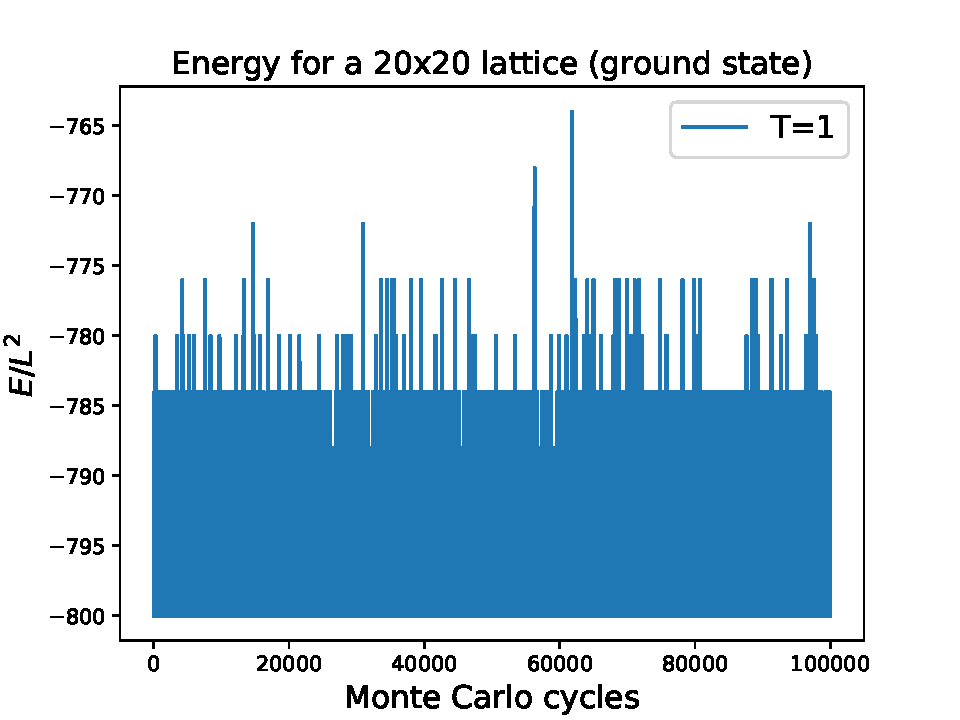
\includegraphics[scale=0.53]{EofMCC-GS-T1-L20-1e5.pdf}}
\subfloat{(a) hva skjer}
}\qquad
{{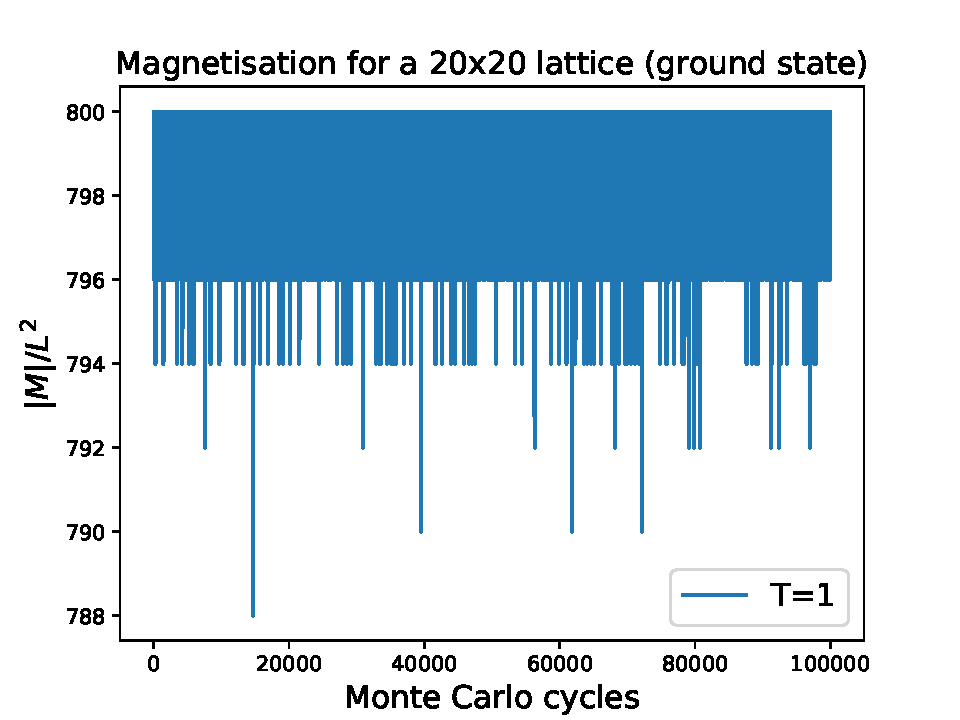
\includegraphics[scale=0.53]{MofMCC-GS-T1-L20-1e5.pdf}}
\subfloat{(b) }
}\qquad
\caption{text}
\label{fig:GS}
\end{figure}

\begin{figure}[H]
{{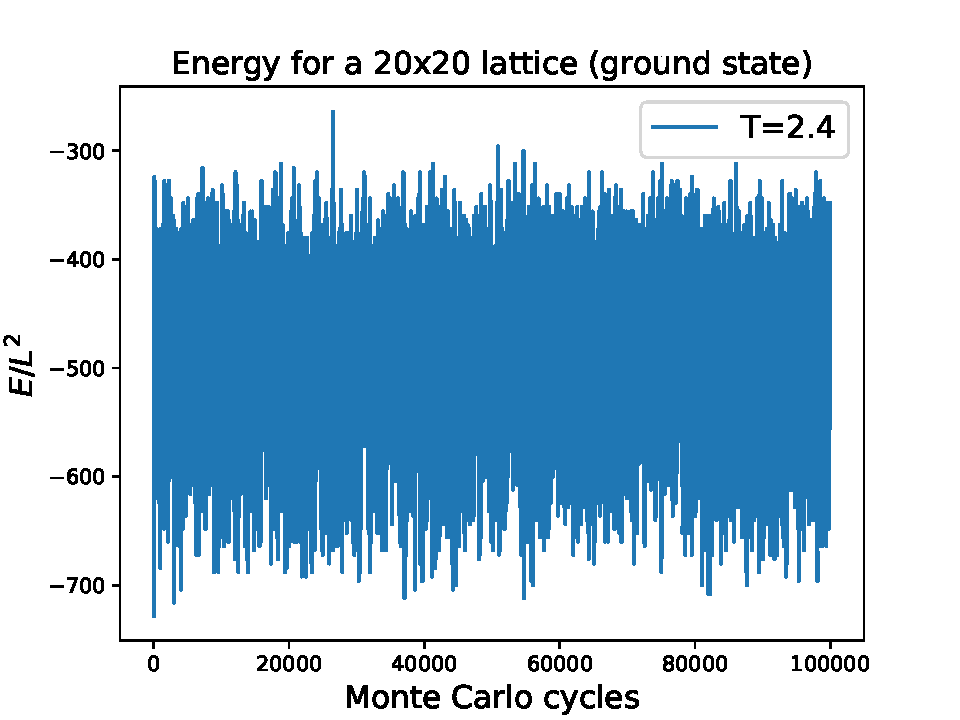
\includegraphics[scale=0.53]{EofMCC-GS-T2_4-L20-1e5.pdf}}
\subfloat{(a) }
}\qquad
{{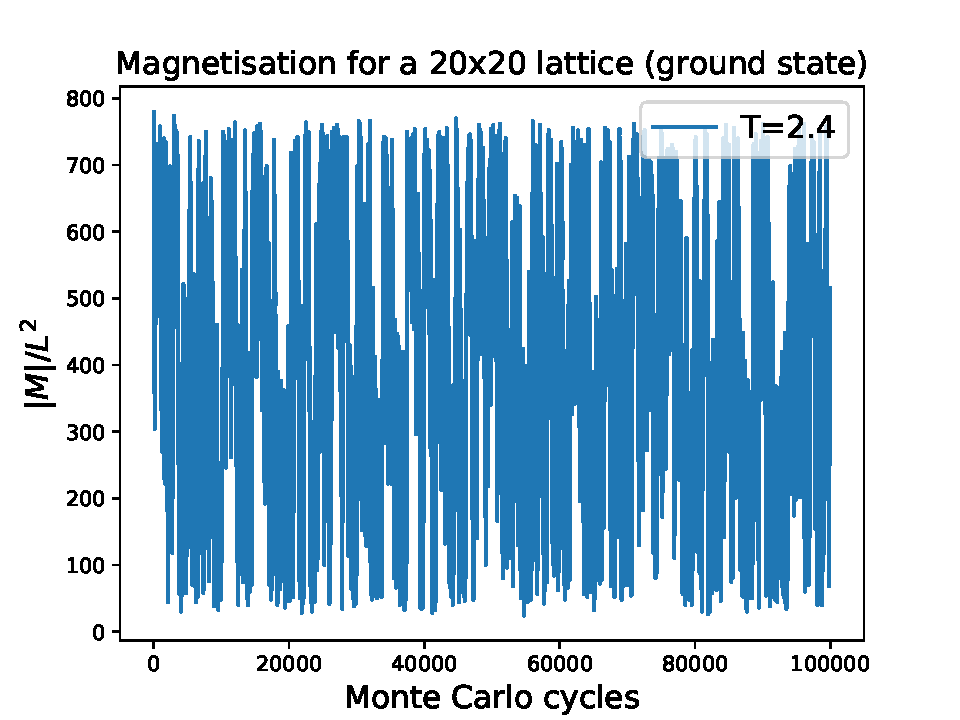
\includegraphics[scale=0.53]{MofMCC-GS-T2_4-L20-1e5.pdf}}
\subfloat{(b) }
}\qquad
\caption{text}
\label{fig:GS}
\end{figure}

\begin{figure}[H]
{{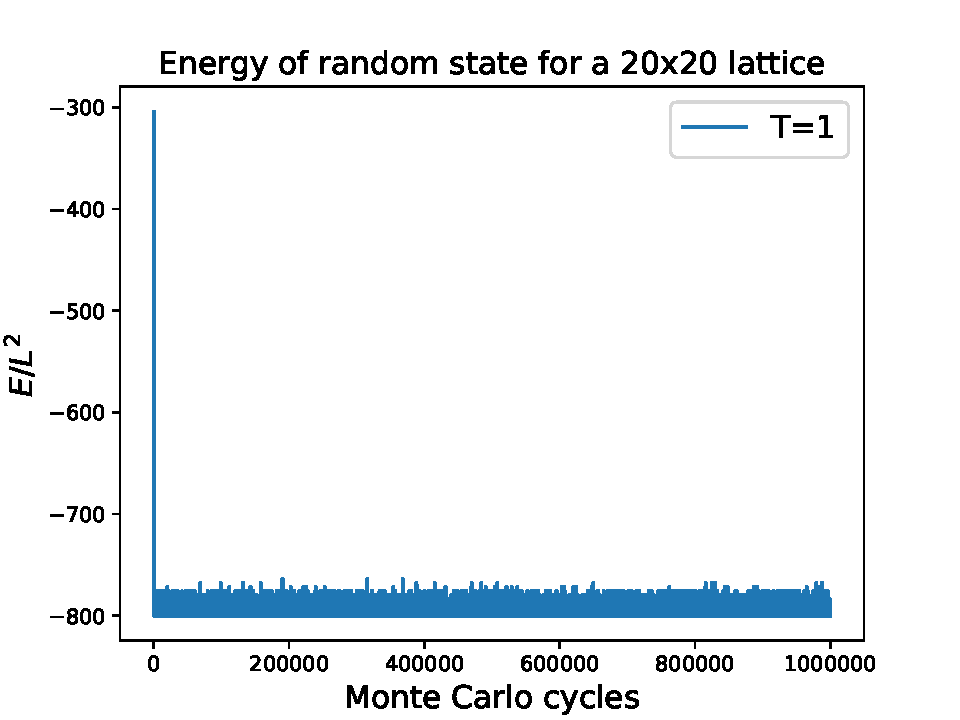
\includegraphics[scale=0.53]{EofMCC-T1-L20-1e6.pdf}}
\subfloat{(a) }
}\qquad
{{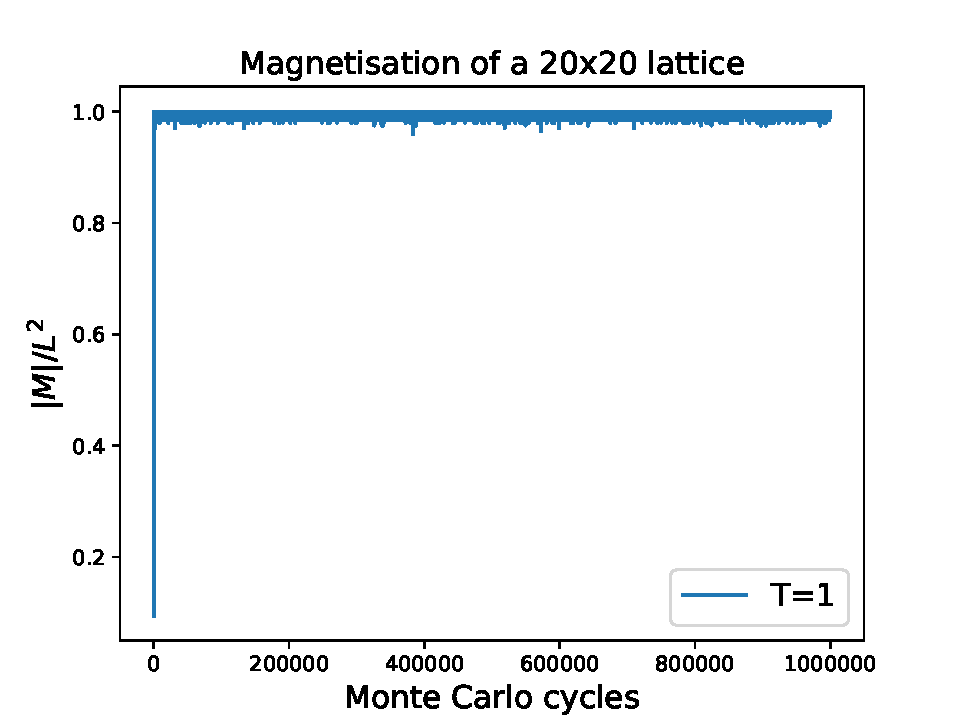
\includegraphics[scale=0.53]{MofMCC-T1-L20-1e6.pdf.pdf}}
\subfloat{(b) }
}\qquad
\caption{text}
\label{fig:GS}
\end{figure}

\begin{figure}[H]
{{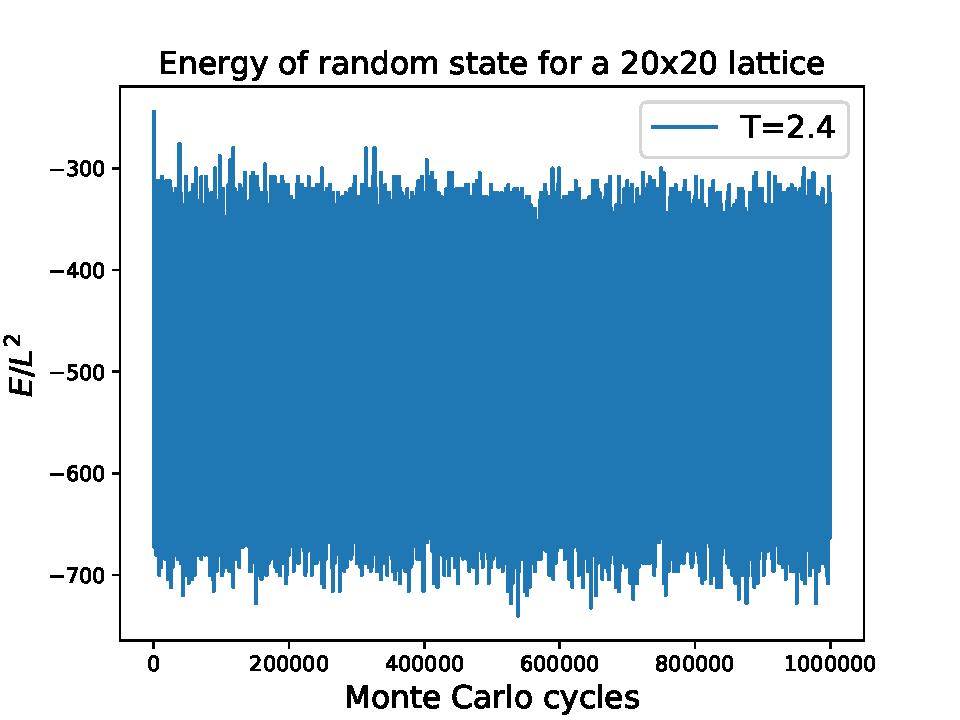
\includegraphics[scale=0.53]{EofMCC-T2_4-L20-1e6.pdf}}
\subfloat{(b) }
}\qquad
{{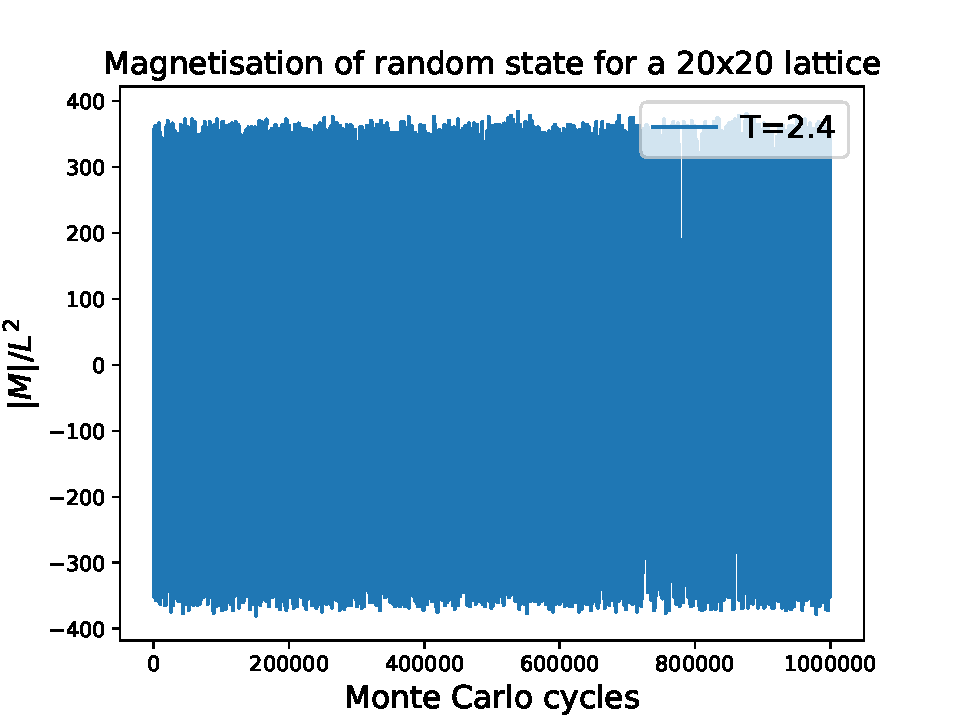
\includegraphics[scale=0.53]{MofMCC-T2_4-L20-1e6.pdf}}
\subfloat{(c) }
}\qquad
\caption{text}
\label{fig:GS}
\end{figure}

\begin{figure}[t]
\mbox{\epsfig{figure=accepts_of_T-T1T2_4-L20.pdf,width=\linewidth,clip=}}
\caption{Description of figure -- explain all elements, but do not
draw conclusions here.}
\label{fig:figure_label}
\end{figure}

\begin{figure}[t]
\mbox{\epsfig{figure=accepts-T1T2_4-L20-1e5.pdf,width=\linewidth,clip=}}
\caption{Description of figure -- explain all elements, but do not
draw conclusions here.}
\label{fig:figure_label}
\end{figure}

\begin{figure}[t]
\mbox{\epsfig{figure=CV-T2-23.pdf,width=\linewidth,clip=}}
\caption{Description of figure -- explain all elements, but do not
draw conclusions here.}
\label{fig:figure_label}
\end{figure}

\begin{figure}[t]
\mbox{\epsfig{figure=CV-T2-23.pdf,width=\linewidth,clip=}}
\caption{Description of figure -- explain all elements, but do not
draw conclusions here.}
\label{fig:figure_label}
\end{figure}

\begin{figure}[t]
\mbox{\epsfig{figure=CV-T22-24.pdf,width=\linewidth,clip=}}
\caption{Description of figure -- explain all elements, but do not
draw conclusions here.}
\label{fig:figure_label}
\end{figure}

\begin{figure}[t]
\mbox{\epsfig{figure=E-T2-23.pdf,width=\linewidth,clip=}}
\caption{Description of figure -- explain all elements, but do not
draw conclusions here.}
\label{fig:figure_label}
\end{figure}

\begin{figure}[t]
\mbox{\epsfig{figure=E-T22-24.pdf,width=\linewidth,clip=}}
\caption{Description of figure -- explain all elements, but do not
draw conclusions here.}
\label{fig:figure_label}
\end{figure}

\begin{figure}[t]
\mbox{\epsfig{figure=FittedTc.pdf,width=\linewidth,clip=}}
\caption{Description of figure -- explain all elements, but do not
draw conclusions here.}
\label{fig:figure_label}
\end{figure}

\begin{figure}[t]
\mbox{\epsfig{figure=M-T2-23.pdf,width=\linewidth,clip=}}
\caption{Description of figure -- explain all elements, but do not
draw conclusions here.}
\label{fig:figure_label}
\end{figure}

\begin{figure}[t]
\mbox{\epsfig{figure=M-T22-24.pdf,width=\linewidth,clip=}}
\caption{Description of figure -- explain all elements, but do not
draw conclusions here.}
\label{fig:figure_label}
\end{figure}

\begin{figure}[t]
\mbox{\epsfig{figure=PE-T1-L20-1e6.pdf,width=\linewidth,clip=}}
\caption{Description of figure -- explain all elements, but do not
draw conclusions here.}
\label{fig:figure_label}
\end{figure}


\begin{figure}[t]
\mbox{\epsfig{figure=PE-T2_4-L20-1e6.pdf,width=\linewidth,clip=}}
\caption{Description of figure -- explain all elements, but do not
draw conclusions here.}
\label{fig:figure_label}
\end{figure}


\begin{figure}[t]
\mbox{\epsfig{figure=X-T2-23.pdf,width=\linewidth,clip=}}
\caption{Description of figure -- explain all elements, but do not
draw conclusions here.}
\label{fig:figure_label}
\end{figure}

\begin{figure}[t]
\mbox{\epsfig{figure=X-T22-24.pdf,width=\linewidth,clip=}}
\caption{Description of figure -- explain all elements, but do not
draw conclusions here.}
\label{fig:figure_label}
\end{figure}





\section{Discussion}
\label{sec:discussion}




\section{Conclusions}
\label{sec:conclusions}




%\begin{figure}[t]
%
%\mbox{\epsfig{figure=filename.eps,width=\linewidth,clip=}}
%
%\caption{Description of figure -- explain all elements, but do not
%draw conclusions here.}
%\label{fig:figure_label}
%\end{figure}



%\begin{deluxetable}{lccc}
%\tablewidth{0pt}
%\tablecaption{\label{tab:results}}
%\tablecomments{Summary of main results.}
%\tablecolumns{4}
%\tablehead{Column 1  & Column 2 & Column 3 & Column 4}
%\startdata
%Item 1 & Item 2 & Item 3 & Item 4
%\enddata
%\end{deluxetable}



\begin{acknowledgements}

\end{acknowledgements}

\begin{thebibliography}{}

\bibitem[G{\'o}rski et al.(1994)]{gorski:1994} G{\'o}rski, K. M.,
  Hinshaw, G., Banday, A. J., Bennett, C. L., Wright, E. L., Kogut,
  A., Smoot, G. F., and Lubin, P.\ 1994, ApJL, 430, 89

\end{thebibliography}


\end{document}
